Vedic astrology, also known as Jyotish, is an ancient system of astrology that originated in the Indian subcontinent. It is considered one of the oldest astrological systems in the world and has its roots in the Vedas, the ancient sacred texts of Hinduism.
Vedic astrology(Jyotish) is one of the most important limb(Vedanga) out of the total six limbs(Vedangas) found in the ancient Indian scriptures. The origins of Vedic astrology can be traced back to around 1500 BCE, during the late Vedic period. It is classified into the three major branches or disciplines known as the Siddhanta, Samhita and Hora. These branches provide different approaches and methods for studying and practicing astrology.

\begin{itemize}
	\item \textbf{Siddhanta:} Siddhanta deals with all the mathematical calculations of space \& time which is involed in the study of planets, stars, comets and contellations present in the space. It is also referred as the Astronomy in modern days.
	\item \textbf{Samhita:} Samhita, also known as Muhurtha, is the branch of Vedic astrology that deals with collective or mundane astrology. It focuses on predicting and analyzing events and phenomena on a broader scale, such as natural disasters, weather patterns, political developments, and societal events.
	\item \textbf{Hora:} Hora or horarian astrology is the branch of Vedic astrology that specifically deals with individual horoscopes or birth charts (Jataka).
\end{itemize}

There are many ancient texts and scriptures about all these three branches of the vedic astrology, that were written by Maharishies. But here, we are only considering the Surya Siddhanta\cite{SuryaSiddhanta, wiki:ss} and Brihat Parashara Hora Shastra\cite{BrihatParasharHoraShastraVol1, BrihatParasharHoraShastraVol2, wiki:bphs} which are the most popular texts that are used by most of the astrologers today for astrological predictions and consultations. We also discuss some of rules and priciples described by the dictums found in these texts.

\subsubsection{Significance of Houses}
The concept of houses plays a significant role in interpreting a person's birth chart or horoscope. The chapters 13 to 24 of Brihat Parashara Hora Shastra\cite{BrihatParasharHoraShastraVol1, BrihatParasharHoraShastraVol2, wiki:bphs} discusses in detail about all these houses. We can understand the concept of the houses by the following dictum:

\begin{sanskrit}
	\begin{center}
		गच्छन्तो भानि गृह्णन्ति सततं ये तु ते ग्रहः।
		भचक्रस्य नगश्व्यंशा अश्विन्यादिसमाह्वयाः॥३:४॥\cite{BrihatParasharHoraShastraVol1, wiki:bphs}\label{Dictum1}\\
		तद्‌द्वादशविभागास्तु तुल्य मेषादिसंज्ञकाः।
		प्रसिद्धा राशयः सन्ति ग्रहास्त्वर्कादिसंज्ञकाः॥३:५॥\cite{BrihatParasharHoraShastraVol1, wiki:bphs}\label{Dictum2}\\
		राशीनामुदयो लग्नं तद्वशादेव जन्मिनाम्‌।
		ग्रहयोग्वियोगाभ्यां फलं चिन्त्यं शुभाशुभम्‌॥३:६॥\cite{BrihatParasharHoraShastraVol1, wiki:bphs}\label{Dictum3}\\
	\end{center}
\end{sanskrit}
The space is divided into twelve houses, also known as "Bhavas," which represent different aspects of an individual's life. Each house is associated with specific areas of life, such as personality traits, relationships, career, wealth, health, spirituality, and more. Here's a brief introduction to the twelve houses in Vedic astrology:

Those planets that constantly move and grab the houses, they are the celestial bodies. The divisions of the zodiac are the angles of the chariot, starting with Ashvini and others.

The twelve divisions are known as equal signs, starting with Aries and others. The well-known zodiac signs are the celestial bodies, starting with the Sun and others.

The rising sign of the zodiac is the Ascendant for individuals. By the combination or separation of the planets, the auspicious and inauspicious results should be contemplated.

\begin{itemize}
	\item \textbf{First House (Lagna or Ascendant):} Represents the self, physical appearance, personality, and overall life path.
	\item \textbf{Second House:} Pertains to wealth, possessions, speech, family, values, and self-worth.
	\item \textbf{Third House:} Governs communication, siblings, skills, short trips, courage, and intellect.
	\item \textbf{Fourth House:} Represents home, mother, comfort, real estate, ancestral property, and emotional foundation.
	\item \textbf{Fifth House:} Relates to creativity, intelligence, children, education, romance, and speculative endeavors.
	\item \textbf{Sixth House:} Deals with health, daily routine, enemies, debts, conflicts, and service to others.
	\item \textbf{Seventh House:} Focuses on partnerships, marriage, relationships, business collaborations, and public image.
	\item \textbf{Eighth House:} Associated with transformations, secrets, inheritances, spirituality, life and death, and occult sciences.
	\item \textbf{Ninth House:} Relates to higher knowledge, beliefs, philosophy, long-distance travel, luck, and spiritual pursuits.
	\item \textbf{Tenth House:} Governs career, reputation, social status, achievements, authority, and public recognition.
	\item \textbf{Eleventh House:} Pertains to gains, friendships, social networks, aspirations, goals, and humanitarian activities.
	\item \textbf{Twelfth House:} Represents solitude, spirituality, hidden enemies, subconscious mind, losses, and liberation.
\end{itemize}

Each house is further influenced by the planetary positions and aspects, providing insights into different areas of life and their interconnections. Analyzing the houses and their interactions helps astrologers interpret a person's life circumstances, potential challenges, and opportunities for growth and fulfillment.

\subsubsection{Properties of Zodiac Signs}
\begin{sanskrit}
	\begin{center}
		अथ खेटा रविश्चन्द्रो मङ्गलश्च बुधस्तथा।\\गुरुः शुक्रः शनि राहुः केतुश्चैते यथाक्रमम्‌॥३:११॥\cite{BrihatParasharHoraShastraVol1, wiki:bphs}\label{Dictum3}
		मेषो वृषश्च मिथुनः कर्कसिंहकुमारिकाः।\\तुलालिऽश्च धनुर्नक्रे कुम्भो मीनस्ततः परम्‌॥४:३॥\cite{BrihatParasharHoraShastraVol1, wiki:bphs}\label{s2}
	\end{center}
\end{sanskrit}
Sun, Moon, Mars, Mercury, Jupiter, Venus, Saturn, Rahu, and Ketu, these are mentioned in order, one by one.\ref{Dictum3}
Aries, Taurus, Gemini, Cancer, Leo, Virgo, Libra, Scorpio, Sagittarius and Pisces are the twelve contellations also known as the zodiac signs.\ref{s2}
However, the main source of all these things are the four basic elements which are the Fire, Water, Wind, Earth \& Sky.
However, describing all the shlokas here is not possible but properties of the twelve zodiac signs are described in shloka number 7 to 23 of BPHS\cite{BrihatParasharHoraShastraVol1, wiki:bphs} which are interpreted by the astrologers as follows:
Aries, Taurus, Gemini, Cancer, Leo, Virgo, Libra, Scorpio, Sagittarius and Pisces.

the zodiac signs are based on the 12 divisions of the ecliptic, with each sign representing a specific portion of the sky. These signs are associated with different elements, ruling planets, qualities, and characteristics that are believed to influence an individual's personality, behavior, and destiny.

Here is a brief introduction to the zodiac signs in Vedic astrology:

Aries (Mesha): The first sign of the zodiac, represented by the Ram. Aries individuals are known for their leadership qualities, courage, and assertiveness.

Taurus (Vrishabha): Symbolized by the Bull, Taurus is associated with stability, determination, practicality, and a strong connection to material possessions and pleasures.

Gemini (Mithuna): Represented by the Twins, Gemini is associated with intellectual pursuits, communication skills, adaptability, and curiosity.

Cancer (Karka): Symbolized by the Crab, Cancer is associated with emotions, sensitivity, nurturing tendencies, and a strong connection to home and family.

Leo (Simha): Represented by the Lion, Leo is associated with creativity, self-expression, leadership, confidence, and a desire for recognition and admiration.

Virgo (Kanya): Symbolized by the Virgin, Virgo is associated with meticulousness, practicality, analytical thinking, attention to detail, and a desire for perfection.

Libra (Tula): Represented by the Scales, Libra is associated with balance, harmony, diplomacy, sociability, and a strong sense of justice.

Scorpio (Vrishchika): Symbolized by the Scorpion, Scorpio is associated with intensity, passion, depth, secrecy, transformation, and a keen sense of intuition.

Sagittarius (Dhanu): Represented by the Archer, Sagittarius is associated with exploration, adventure, intellectual pursuits, optimism, and a philosophical outlook on life.

Capricorn (Makara): Symbolized by the Goat, Capricorn is associated with discipline, ambition, responsibility, practicality, and a strong drive for success.

Aquarius (Kumbha): Represented by the Water Bearer, Aquarius is associated with humanitarianism, independence, innovation, intellectual pursuits, and a desire for social change.

Pisces (Meena): Symbolized by the Fish, Pisces is associated with sensitivity, intuition, empathy, imagination, spirituality, and a strong connection to the subconscious realm.

These zodiac signs play a crucial role in Vedic astrology, serving as a foundation for determining individual traits, compatibility between individuals, and making predictions about various aspects of life, including career, relationships, health, and spiritual growth.

\subsubsection{Properties of Planets}
\begin{sanskrit}
	\begin{center}
		सर्वात्मा च दीवानाथो मनः कुमुदबान्धवः।\\सत्त्वं कुजो बुधैः प्रोक्तो बुधो वाणीप्रदायकः॥३:१३॥\cite{BrihatParasharHoraShastraVol1, wiki:bphs}
	\end{center}
\end{sanskrit}
\begin{sanskrit}
	\begin{center}
		देवेज्यो ज्ञानसुखदो भृगुर्वीर्यप्रदयकः।\\ऋषिभिः प्राक्‌तनैः प्रोक्तश्छायासूनुश्च दुःखदः॥३:१४॥\cite{BrihatParasharHoraShastraVol1, wiki:bphs}
	\end{center}
\end{sanskrit}
Jupiter(Brihaspati) is the significator of wisdom. 
Venus(Shukra) is resposible for joy \& ecstacy.
\begin{sanskrit}
	\begin{center}
		रविचन्द्रौ तु राजानौ नेता ज्ञेयो धरात्मजः।\\बुधो राजकुमारश्च सचिवौ गुरुभार्गवौ॥३:१५॥\cite{BrihatParasharHoraShastraVol1, wiki:bphs}
	\end{center}
\end{sanskrit}
Mars(Mangal) is responsible for the strength of a native which leads to the emotion of anger.
Rahu

the study of planets holds great significance in understanding an individual's horoscope and predicting future events. Vedic astrology recognizes nine celestial bodies as planets, including the Sun, Moon, Mercury, Venus, Mars, Jupiter, Saturn, Rahu, and Ketu. Here's a brief introduction to each of these planets in the context of Vedic astrology:

Sun (Surya): The Sun represents the self, vitality, authority, and leadership. It symbolizes the soul and is considered the king among the planets.

Moon (Chandra): The Moon represents emotions, mind, instincts, and nurturing qualities. It influences the individual's emotional well-being and intuition.

Mercury (Budha): Mercury is associated with communication, intellect, logic, and adaptability. It governs speech, learning, and mental abilities.

Venus (Shukra): Venus is the planet of love, beauty, art, and harmony. It governs relationships, attraction, creativity, and material pleasures.

Mars (Mangal): Mars signifies energy, passion, courage, and assertion. It governs ambition, drive, physical strength, and competitiveness.

Jupiter (Guru): Jupiter is considered the most benefic planet in Vedic astrology. It represents wisdom, knowledge, expansion, abundance, and spirituality.

Saturn (Shani): Saturn is associated with discipline, responsibility, hard work, and karmic lessons. It teaches patience, endurance, and signifies limitations and life challenges.

Rahu: Rahu is a shadow planet and represents material desires, obsession, illusions, and worldly attachments. It signifies ambition and can bring sudden changes.

Ketu: Ketu is the other shadow planet and represents spirituality, detachment, mysticism, and karmic lessons. It signifies liberation and can bring unconventional experiences.

Each planet's placement, aspects, and interactions with other planets in an individual's birth chart play a crucial role in determining their personality traits, strengths, challenges, and life events according to Vedic astrology.

\subsubsection{Dashas \& Transits}
\begin{sanskrit}
	\begin{center}
		विकलानाम् कला षष्ट्या तत्षष्ट्या भाग उच्यते।\\तत्त्रिम्शता भवेद् राशिर् भगणो द्वादशैव ते॥१:२८॥\cite{SuryaSiddhanta, wiki:ss}
	\end{center}
\end{sanskrit}
60 Vikalas make one kala and 60 kalas make one degree(\textdegree) or one amsa. 30\textdegree(degrees or amsa) make one rashi(one zodiac sign) and twelve such rashies(zodiac signs) make one revolution(bhagana) of the zodiac.

\noindent
\begin{table}[H]
	\begin{tabularx}{\columnwidth}{|M|M|M|}
		\hline
		\textbf{Graha(Planet)} & \textbf{Angular Speed(\textdegree/Day)} & \textbf{Time For One Zodiac Sign} \\
		\hline
		Surya(Sun) & 1 & 1 Month \\
		\hline
		Chandra(Moon) & 13 & 2.25 Days \\
		\hline
		Brihaspati(Jupiter) & 1/12 & 1 Year \\
		\hline
		Shani(Saturn) & 1/30 & 2.5 Years \\
		\hline
		Budh(Mercury) & 1 & 1 Month \\
		\hline
		Shukra(Venus) & 1 & 1 Month \\
		\hline
		Mangal(Mars) & 2/3 & 1.5 Month \\
		\hline
		Rahu & -1/18 & 18 Months \\
		\hline
		Ketu & -1/18 & 18 Months \\
		\hline
	\end{tabularx}
	\caption{Time required by all planets to complete one zodiac sign}
	\label{Table:table}
\end{table}

Table \ref{Table:table} represents the time required by all nine planets to complete one zodiac sign which is calculated in chapter 1, verse 29 to 34 of Surya Siddhanta\cite{SuryaSiddhanta, wiki:ss}.

Effect of dashaas of the different planets in Chapter number 53 of BPHS.

The planetary vibrations reflected or refracted along with solar radiations to the earth are of varying intensities as per planetary distance, size, and movement in the solar system. These vibrations impact our sensory nerves, mental attitudes, and moods. Thus, it’s very likely that these planetary vibrations supply the energies to the body cells though our nerves. Since these vibrations differ in wavelength intensity and frequency as per the planetary properties and motion; these vibrations supply different sensory stimuli which impacts the human unconscious and personality at the time of birth\cite{article}.
\\\\\\\\
Planetary positions influence on psychology

Vedic astrology, also known as Jyotish, is an ancient system of astrology that originated in the Indian subcontinent. It is considered one of the oldest astrological systems in the world and has its roots in the Vedas, the ancient sacred texts of Hinduism.
Vedic astrology is one of the most important limb(Vedanga) out of the total six limbs(Vedangas) found in the ancient Indian scriptures. The origins of Vedic astrology can be traced back to around 1500 BCE, during the late Vedic period. It is classified into the three major branches or disciplines known as the Siddhanta, Samhita and Hora. These branches provide different approaches and methods for studying and practicing astrology.
\begin{itemize}
	\item \textbf{Siddhanta:} Siddhanta deals with all the mathematical calculations of space \& time which is involed in the study of planets, stars, comets and contellations present in the space. It is also referred as the Astronomy in modern days.
	\item \textbf{Samhita:} Samhita, also known as Muhurtha, is the branch of Vedic astrology that deals with collective or mundane astrology. It focuses on predicting and analyzing events and phenomena on a broader scale, such as natural disasters, weather patterns, political developments, and societal events.
	\item \textbf{Hora:} Hora or horarian astrology is the branch of Vedic astrology that specifically deals with individual horoscopes or birth charts (Jataka).
\end{itemize}

\begin{sanskrit}
	\begin{center}
		अथ खेटा रविश्चन्द्रो मङ्गलश्च बुधस्तथा।\\गुरुः शुक्रः शनि राहुः केतुश्चैते यथाक्रमम्‌॥३:११॥\cite{BrihatParasharHoraShastraVol1}\cite{wiki:bphs}\label{s1}
		मेषो वृषश्च मिथुनः कर्कसिंहकुमारिकाः।\\तुलालिऽश्च धनुर्नक्रे कुम्भो मीनस्ततः परम्‌॥४:३॥\cite{BrihatParasharHoraShastraVol1}\cite{wiki:bphs}\label{s2}
	\end{center}
\end{sanskrit}
Sun, Moon, Mars, Mercury, Jupiter, Venus, Saturn, Rahu, and Ketu, these are mentioned in order, one by one.\ref{s1}
Aries, Taurus, Gemini, Cancer, Leo, Virgo, Libra, Scorpio, Sagittarius and Pisces are the twelve contellations also known as the zodiac signs.\ref{s2}
However, the main source of all these things are the four basic elements which are the Fire, Water, Wind, Earth \& Sky.

\subsubsection{Significance of Houses}

\subsubsection{Properties of Zodiac Signs}
However, describing all the shlokas here is not possible but properties of the twelve zodiac signs are described in shloka number 7 to 23 of BPHS\cite{BrihatParasharHoraShastraVol1}\cite{wiki:bphs} which are interpreted by the astrologers as follows:
Aries, Taurus, Gemini, Cancer, Leo, Virgo, Libra, Scorpio, Sagittarius and Pisces.

\subsubsection{Properties of Planets}
\begin{sanskrit}
	\begin{center}
		सर्वात्मा च दीवानाथो मनः कुमुदबान्धवः।\\सत्त्वं कुजो बुधैः प्रोक्तो बुधो वाणीप्रदायकः॥३:१३॥\cite{BrihatParasharHoraShastraVol1}\cite{wiki:bphs}
	\end{center}
\end{sanskrit}
\begin{sanskrit}
	\begin{center}
		देवेज्यो ज्ञानसुखदो भृगुर्वीर्यप्रदयकः।\\ऋषिभिः प्राक्‌तनैः प्रोक्तश्छायासूनुश्च दुःखदः॥३:१४॥\cite{BrihatParasharHoraShastraVol1}\cite{wiki:bphs}
	\end{center}
\end{sanskrit}
Jupiter(Brihaspati) is the significator of wisdom. 
Venus(Shukra) is resposible for joy \& ecstacy.
\begin{sanskrit}
	\begin{center}
		रविचन्द्रौ तु राजानौ नेता ज्ञेयो धरात्मजः।\\बुधो राजकुमारश्च सचिवौ गुरुभार्गवौ॥३:१५॥\cite{BrihatParasharHoraShastraVol1}\cite{wiki:bphs}
	\end{center}
\end{sanskrit}
Mars(Mangal) is responsible for the strength of a native which leads to the emotion of anger.
Rahu
\subsubsection{Combinations of Planets with Zodiac Signs}
Effect of different combinations of planets along with the zodiac signs on psychology of human emotions.
However, instead of considering the zodiac signs, one can consider the 27 nakshatras for detailed calculations but for simplicity, we are considering the zodiacs here.
\subsubsection{Dashas \& Transits}
\begin{sanskrit}
	\begin{center}
		विकलानाम् कला षष्ट्या तत्षष्ट्या भाग उच्यते।\\तत्त्रिम्शता भवेद् राशिर् भगणो द्वादशैव ते॥१:२८॥\cite{SuryaSiddhanta}\cite{wiki:ss}
	\end{center}
\end{sanskrit}
60 Vikalas make one kala and 60 kalas make one degree(\textdegree) or one amsa. 30\textdegree(degrees or amsa) make one rashi(one zodiac sign) and twelve such rashies(zodiac signs) make one revolution(bhagana) of the zodiac.

\begin{table}[H]
	\begin{tabular}{|c|c|c|}
		\hline
		\textbf{Graha} & \textbf{Angular Speed} & \textbf{Time For One} \\
		\textbf{(Planet)} & \textbf{(\textdegree/Day)} & \textbf{Zodiac Sign}\\
		\hline
		Surya(Sun) & 1 & 1 Month \\
		\hline
		Chandra(Moon) & 13 & 2.25 Days \\
		\hline
		Brihaspati(Jupiter) & 1/12 & 1 Year \\
		\hline
		Shani(Saturn) & 1/30 & 2.5 Years \\
		\hline
		Budh(Mercury) & 1 & 1 Month \\
		\hline
		Shukra(Venus) & 1 & 1 Month \\
		\hline
		Mangal(Mars) & 2/3 & 1.5 Month \\
		\hline
		Rahu & -1/18 & 18 Months \\
		\hline
		Ketu & -1/18 & 18 Months \\
		\hline
	\end{tabular}
	\caption{Time required by all planets to complete one zodiac sign}
	\label{Table:table}
\end{table}

Table \ref{Table:table} represents the time required by all nine planets to complete one zodiac sign which is calculated in chapter 1, verse 29 to 34 of Surya Siddhanta\cite{SuryaSiddhanta}\cite{wiki:ss}.

Effect of dashaas of the different planets in Chapter number 53 of BPHS.

The planetary vibrations reflected or refracted along with solar radiations to the earth are of varying intensities as per planetary distance, size, and movement in the solar system. These vibrations impact our sensory nerves, mental attitudes, and moods. Thus, it’s very likely that these planetary vibrations supply the energies to the body cells though our nerves. Since these vibrations differ in wavelength intensity and frequency as per the planetary properties and motion; these vibrations supply different sensory stimuli which impacts the human unconscious and personality at the time of birth\cite{article}.
\subsubsection{Sudarshan Chakra}
\begin{sanskrit}
	\begin{center}
		जन्मतो मृत्युपर्यन्तं वर्षमासदिनोद्भवम्।\\शुभं वाऽप्यशुभं सर्वं तच्छृणुष्वैकमानसः॥७४:४॥\cite{BrihatParasharHoraShastraVol2}\cite{wiki:bphs}
	\end{center}
\end{sanskrit}
Physical Level
Mental Level
Spiritual Level
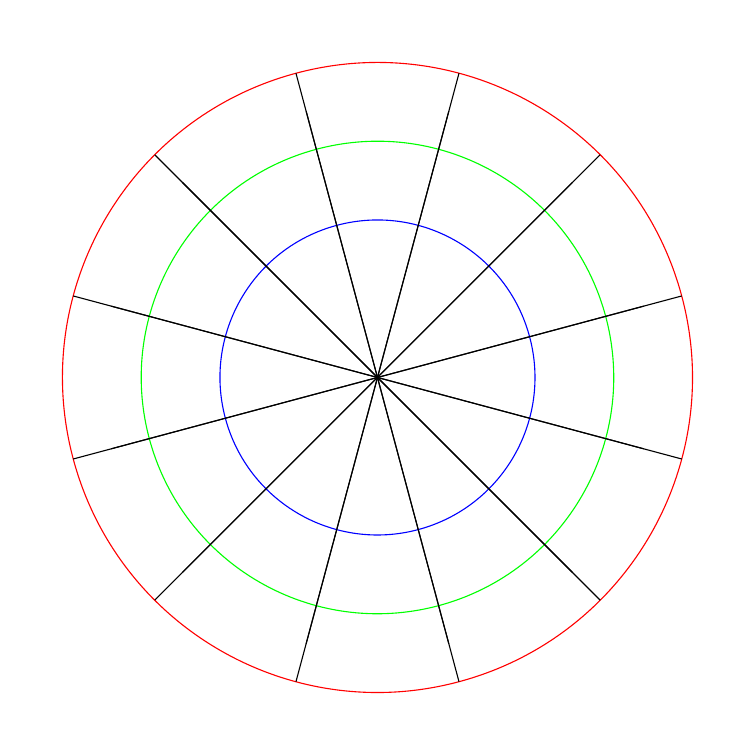
\begin{tikzpicture}[rotate=15]
	\definecolor{mycolor1}{RGB}{255,0,0}
	\definecolor{mycolor2}{RGB}{0,255,0}
	\definecolor{mycolor3}{RGB}{0,0,255}
	\draw[mycolor1] (0,0) circle (4cm);
	\draw[mycolor2] (0,0) circle (3cm);
	\draw[mycolor3] (0,0) circle (2cm);
	\foreach \i in {0,30,...,330}
	{
		\draw (\i:3.5cm) -- (\i+180:4cm);
	}
\end{tikzpicture}
